\chapter{Application design}\label{ch:design}

The application is divided into three components:
\begin{itemize}
	\item[\standout{Common}] A library that contains modules that are used
		both by the server and the client. This includes the protocol
		implementation, networking functions, PEM serialization, error
		reporting, console output, \etc; Its code is available in the
		\code{common} folder;
	\item[\standout{Server}] The server application which handles the
		registered users allowing them to log-in and challenge each
		other. Its code is available in the \code{server} folder;
	\item[\standout{Client}] The client application that is used by the user
		to log-in with the server and play the game against other
		players. Its code is available in the \code{client} folder.
\end{itemize}

Each components is divided into a number of modules. Each module provides
functions for a specific functionality of the application and it's compound by a
\emph{C source file} and a \emph{Header file}. All header files are placed under
the \code{include} directory.

\figref{fig:modules} shows all the modules of the developed application along
with their connections with other modules\footnote{Only the main connections are
represented.}.

\begin{figure}[htb]
	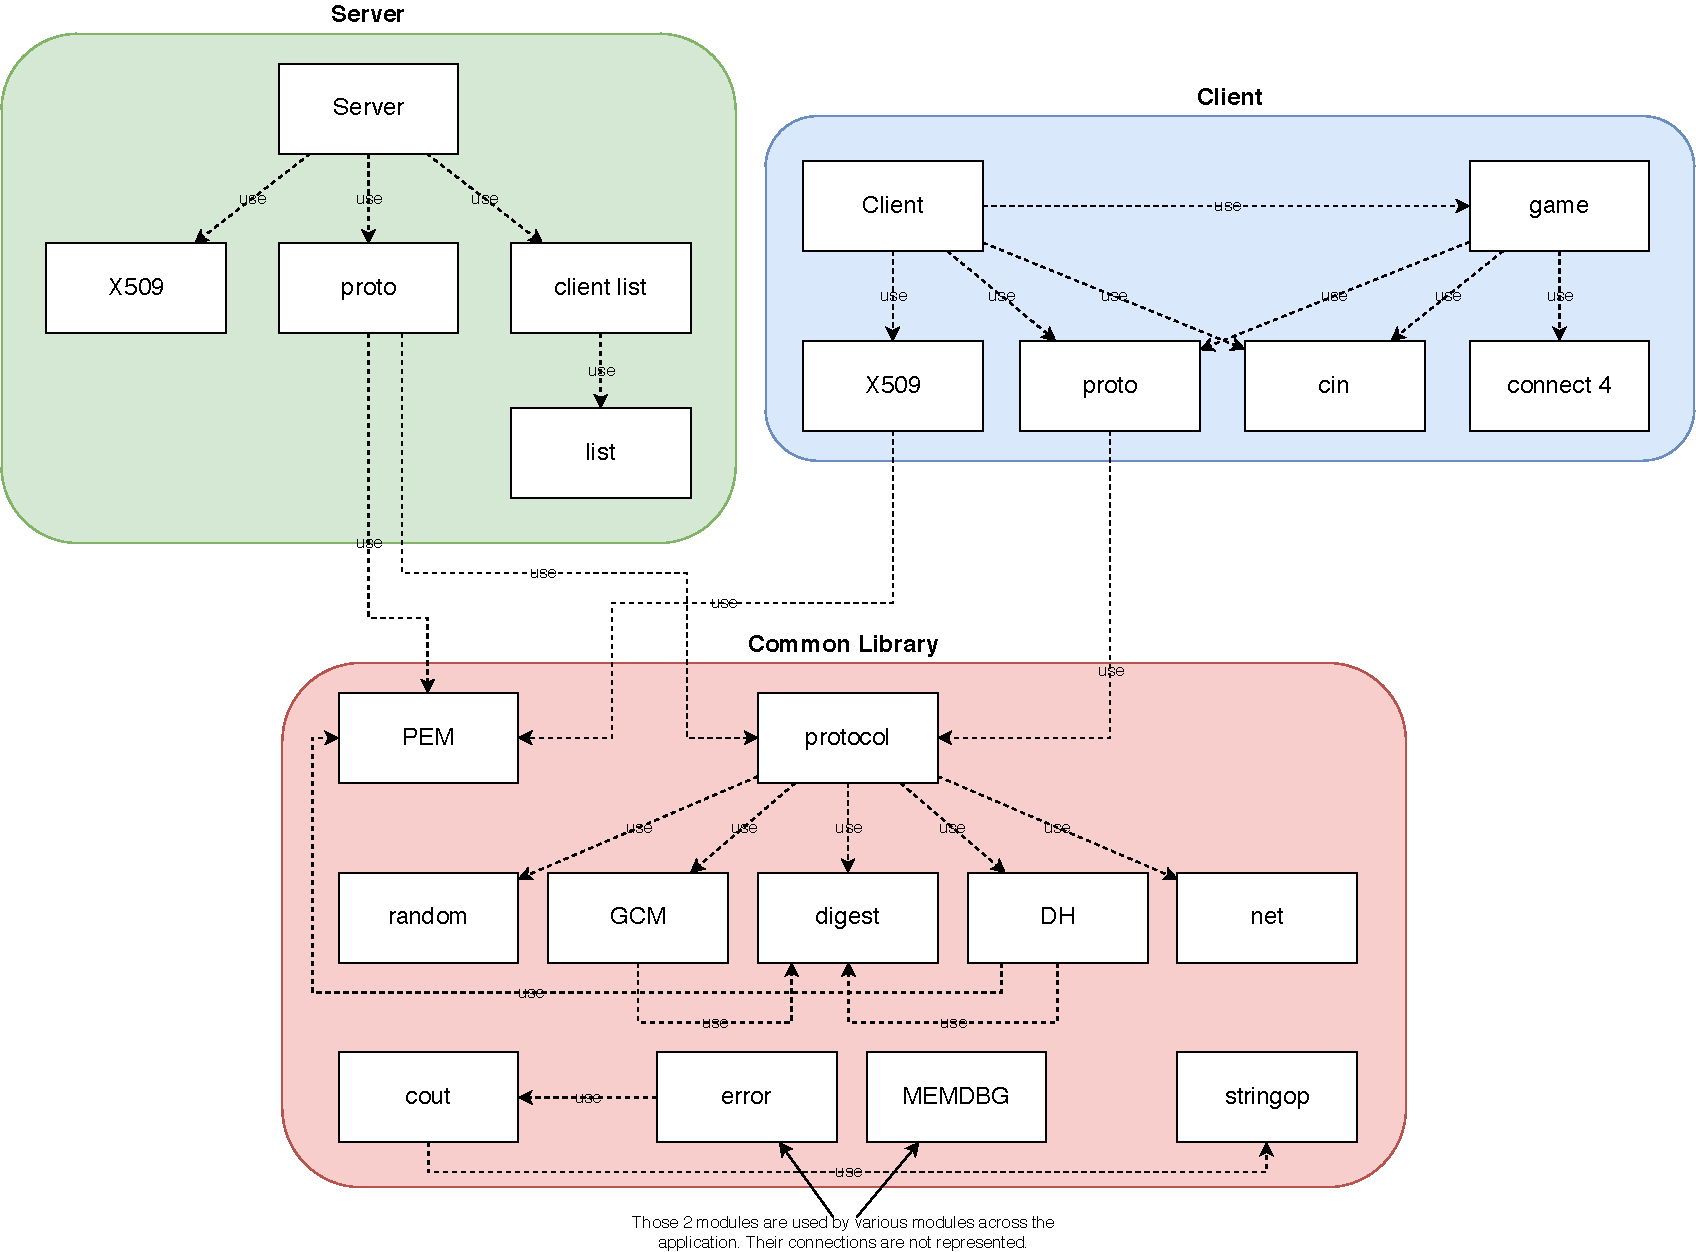
\includegraphics[width=\textwidth]{modules}
	\caption{Application modules}\label{fig:modules}
\end{figure}

\section{Common library modules}\label{sec:commonmod}

\ldots

\subsection{Protocol modules}\label{subsec:protomods}

\ldots

\subsubsection{Networking (net)}

\ldots

\subsubsection{Digest}

\ldots

\subsubsection{Diffie-Hellman (DH)}

\ldots

\subsubsection{GCM}

\ldots

\subsection{Other modules}\label{subsec:othermods}

\ldots

\subsubsection{PEM}

\ldots

\subsubsection{Random}

\ldots

\subsubsection{Console output (cout)}

\ldots

\subsubsection{String operations (stringop)}

\ldots

\subsubsection{Error reporting (error)}

\ldots

\subsubsection{MEMDBG}

\ldots


\section{Client-Server}\label{sec:servermsgs}

\begin{itemize}
	\item[] \standout{CLIENT\_HELLO} \emph{(signed)} The message sent by the
		client to the server at the beginning of the session. It carries
		the username of the client, and the port where the client can be
		contacted by other clients to start a game.
	\item[] \standout{SERVER\_CERT} \emph{(plain)} The message sent by the
		server to the client containing its own certificate.
	\item[] \standout{SERVER\_HELLO} \emph{(signed)} The message sent by the
		server to the client in response to a \code{CLIENT\_HELLO}
		message. It contains the same username received in the
		\code{CLIENT\_HELLO} message.
	\item[] \standout{DHKEY} \emph{(signed)} The message sent by the client
		to the server and vice versa that contains the
		\emph{Diffie-Hellman} public key used to derive a shared secret.
	\item[] \standout{PLAYER\_LIST\_REQ} \emph{(encrypted)} This empty
		message is sent by the client to the server when the client
		wants to get the list of the currently logged-in players.
	\item[] \standout{PLAYER\_LIST} \emph{(encrypted)} The reply message
		from the server to the client containing the list of all the
		users connected to the system.
	\item[] \standout{CHALLENGE\_REQ} \emph{(encrypted)} The message sent
		from a client to the server containing the username of the
		challenged user.
	\item[] \standout{CHALLENGE\_RES} \emph{(encrypted)} The message sent by
		the challenged client to the server containing a boolean that it
		is \emph{true} if the user has accepted the challenge.
	\item[] \standout{CLIENT\_INFO} \emph{(encrypted)} The message sent by
		the server to the parties that are starting a new game. It
		contains the \emph{address}, the \emph{game port}, the
		\emph{public key} of the peer and the nonce value to use in the
		\textit{Diffie-Hellman} key exchange.
	\item[] \standout{GAME\_END} \emph{(encrypted)} The message sent by the
		client to the server when the game in which he was engaged ends.
	\item[] \standout{ERROR} The message sent from the server to a client or
		vice versa containing an error code and an error message.
\end{itemize}

\section{Client modules}\label{sec:clientmod}

\ldots

\subsection{X509}\label{subsec:clientx509mod}

\ldots

\subsection{Proto}\label{subsec:clientprotomod}

\ldots

\subsection{Console input (cin)}\label{subsec:cinmod}

\ldots

\subsection{Main module}\label{subsec:clientmainmod}

\ldots

\subsection{Game modules}\label{subsec:gamemods}

\ldots

\subsubsection{Connect 4}

\ldots

\subsubsection{Peer-to-Peer game (game)}

\ldots

